\documentclass[../main.tex]{subfiles}

\begin{document}
\chapter{Roots: Bracketing Methods}
\label{chap:chap5}

\begin{center}
    \Large{\textbf{CHAPTER OBJECTIVES}}
\end{center}
The primary objective of this chapter is to acquaint you with bracketing methods for
finding the root of a single nonlinear equation. Specific objectives and topics covered are

\begin{itemize}
\item Understanding what roots problems are and where they occur in engineering and
science.
\item Knowing how to determine a root graphically.
\item Understanding the incremental search method and its shortcomings.
\item Knowing how to solve a roots problem with the bisection method.
\item Knowing how to estimate the error of bisection and why it differs from error
estimates for other types of root-location algorithms.
\item Understanding false position and how it differs from bisection.
\end{itemize}
\bigskip

\noindent\textbf{YOU'VE GOT A PROBLEM}\\

\noindent Medical studies have established that a bungee jumper's chances of sustaining a
significant vertebrae injury increase significantly if the free-fall velocity exceeds
36 m/s after 4 s of free fall. Your boss at the bungee-jumping company wants you
to determine the mass at which this criterion is exceeded given a drag coefficient of
0.25 kg/m.

You know from your previous studies that the following analytical solution can be
used to predict fall velocity as a function of time:\\

$v(t)=\sqrt{\dfrac{gm}{c_d}}$tanh$(\sqrt{\dfrac{gc_d}{m}}t)$
\hfill (5.1)\\

\noindent
Try as you might, you cannot manipulate this equation to explicitly solve for $m$---that is,
you cannot isolate the mass on the left side of the equation.

An alternative way of looking at the problem involves subtracting v(t) from both sides
to give a new function:\\

$f(m)=\sqrt{\dfrac{gm}{c_d}}$tanh$(\sqrt{\dfrac{gc_d}{m}}t)-v(t)$
\hfill (5.2)\\

\noindent Now we can see that the answer to the problem is the value of $m$ that makes the function
equal to zero. Hence, we call this a ``roots'' problem. This chapter will introduce you to how
the computer is used as a tool to obtain such solutions.\\

\section[ROOTS IN ENGINEERING AND SCIENCE]{ROOTS IN ENGINEERING AND SCIENCE}
\noindent Although they arise in other problem contexts, roots of equations frequently occur in the
area of design. Table 5.1 lists a number of fundamental principles that are routinely used in
design work. As introduced in Chap. 1, mathematical equations or models derived from
these principles are employed to predict dependent variables as a function of independent
variables, forcing functions, and parameters. Note that in each case, the dependent variables
reflect the state or performance of the system, whereas the parameters represent its
properties or composition.

An example of such a model is the equation for the bungee jumper's velocity. If the parameters
are known, Eq. (5.1) can be used to predict the jumper's velocity. Such computations
can be performed directly because $v$ is expressed \emph{explicitly} as a function of the model
parameters. That is, it is isolated on one side of the equal sign.

However, as posed at the start of the chapter, suppose that we had to determine the
mass for a jumper with a given drag coefficient to attain a prescribed velocity in a set time
period. Although Eq. (5.1) provides a mathematical representation of the interrelationship
among the model variables and parameters, it cannot be solved explicitly for mass. In such
cases, $m$ is said to be $implicit$.\\

\begin{figure}[h]
    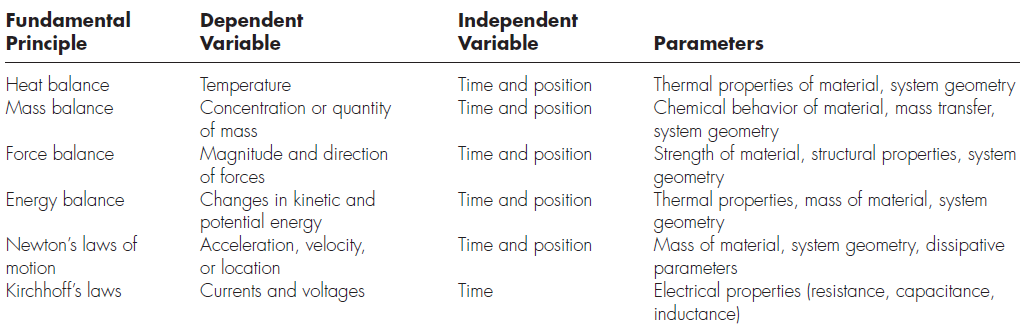
\includegraphics[width=0.9\linewidth]{./images/table_5_1}
\end{figure}

This represents a real dilemma, because many design problems involve specifying the
properties or composition of a system (as represented by its parameters) to ensure that it
performs in a desired manner (as represented by its variables). Thus, these problems often
require the determination of implicit parameters.

The solution to the dilemma is provided by numerical methods for roots of equations.
To solve the problem using numerical methods, it is conventional to reexpress Eq. (5.1) by
subtracting the dependent variable v from both sides of the equation to give Eq. (5.2). The
value of m that makes $f (m) = 0$ is, therefore, the root of the equation. This value also represents
the mass that solves the design problem.

The following pages deal with a variety of numerical and graphical methods for determining
roots of relationships such as Eq. (5.2). These techniques can be applied to many
other problems confronted routinely in engineering and science.\\

\section[GRAPHICAL METHODS]{GRAPHICAL METHODS}
\noindent A simple method for obtaining an estimate of the root of the equation $f(x) = 0$ is to make
a plot of the function and observe where it crosses the $x$ axis. This point, which represents
the $x$ value for which $f(x) = 0$, provides a rough approximation of the root.\\

\begin{example} The Graphical Approach\\

    \noindent\textbf{Problem Statement.}\quad Use the graphical approach to determine the mass of the bungee
    jumper with a drag coefficient of 0.25 kg/m to have a velocity of 36 m/s after 4 s of free
    fall. Note: The acceleration of gravity is $9.81 m/s^2$.\\

    \noindent\textbf{Solution.}\quad The following MATLAB session sets up a plot of Eq. (5.2) versus mass:\\

    \texttt{>> cd = 0.25; g = 9.81; v = 36; t = 4;\\
    \indent >> mp = linspace(50,200);\\
    \indent >> fp = sqrt(g*mp/cd).*tanh(sqrt(g*cd./mp)*t)-v;\\
    \indent >> plot(mp,fp),grid}\\

    The function crosses the $m$ axis between 140 and 150 kg. Visual inspection of the plot
    provides a rough estimate of the root of 145 kg (about 320 lb). The validity of the graphical
    estimate can be checked by substituting it into Eq. (5.2) to yield\\

    \texttt{>> sqrt(g*145/cd)*tanh(sqrt(g*cd/145)*t)-v\\
    \indent ans =\\
    \indent\indent 0.0456}\\

    \noindent which is close to zero. It can also be checked by substituting it into Eq. (5.1) along with the
    parameter values from this example to give\\

    \texttt{>> sqrt(g*145/cd)*tanh(sqrt(g*cd/145)*t)\\
    \indent ans =\\
    \indent\indent 36.0456}\\

    \noindent which is close to the desired fall velocity of 36 m/s.

    \begin{figure}[h]
        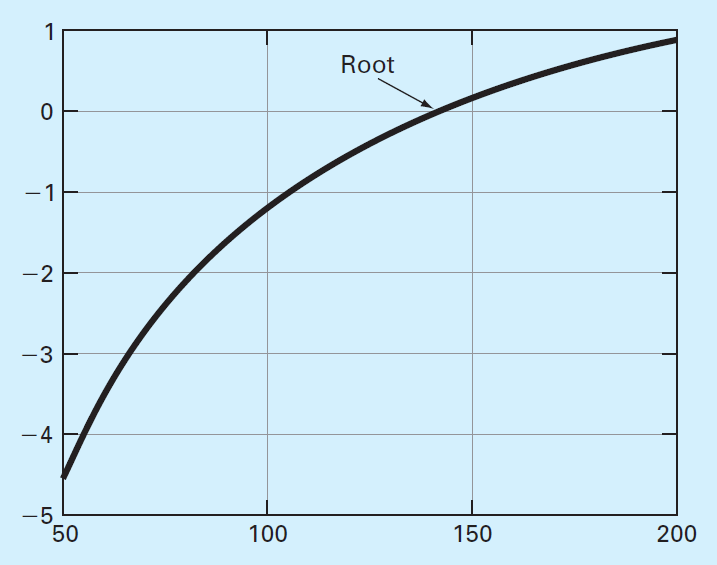
\includegraphics[width=0.7\linewidth]{./images/fig_5_0}
    \end{figure}
\end{example}

Graphical techniques are of limited practical value because they are not very precise.
However, graphical methods can be utilized to obtain rough estimates of roots. These estimates
can be employed as starting guesses for numerical methods discussed in this chapter.

Aside from providing rough estimates of the root, graphical interpretations are useful for
understanding the properties of the functions and anticipating the pitfalls of the numerical
methods. For example, Fig. 5.1 shows a number of ways in which roots can occur (or be
absent) in an interval prescribed by a lower bound $x_l$ and an upper bound $x_u$. Figure 5.1b depicts
the case where a single root is bracketed by negative and positive values of f (x). However,
Fig. 5.1d, where $f(x_l)$ and $f(x_u)$ are also on opposite sides of the x axis, shows three
roots occurring within the interval. In general, if $f(x_l)$ and $f(x_u)$ have opposite signs, there
are an odd number of roots in the interval. As indicated by Fig. 5.1a and c, $if f(x_l)$ and $f (x_u)$
have the same sign, there are either no roots or an even number of roots between the values.

Although these generalizations are usually true, there are cases where they do not hold.
For example, functions that are tangential to the $x$ axis (Fig. 5.2a) and discontinuous functions
(Fig. 5.2b) can violate these principles. An example of a function that is tangential to
the axis is the cubic equation $f (x) = (x - 2)(x - 2)(x - 4)$. Notice that $x = 2$ makes two
terms in this polynomial equal to zero. Mathematically, $x = 2$ is called a \emph{multiple root}.
Although they are beyond the scope of this book, there are special techniques that are
expressly designed to locate multiple roots (Chapra and Canale, 2010).

The existence of cases of the type depicted in Fig. 5.2 makes it difficult to develop foolproof
computer algorithms guaranteed to locate all the roots in an interval. However, when
used in conjunction with graphical approaches, the methods described in the following sections
are extremely useful for solving many problems confronted routinely by engineers,
scientists, and applied mathematicians.\\

\section[BRACKETING METHODS AND INITIAL GUESSES]{BRACKETING METHODS AND INITIAL GUESSES}
\noindent If you had a roots problem in the days before computing, you'd often be told to use ``trial and
error'' to come up with the root. That is, you'd repeatedly make guesses until the function
was sufficiently close to zero. The process was greatly facilitated by the advent of software tools such as spreadsheets.

\noindent By allowing you to make many guesses rapidly, such tools can
actually make the trial-and-error approach attractive for some problems.

But, for many other problems, it is preferable to have methods that come up with the
correct answer automatically. Interestingly, as with trial and error, these approaches require
an initial ``guess'' to get started. Then they systematically home in on the root in an iterative
fashion.

The two major classes of methods available are distinguished by the type of initial
guess. They are

\begin{itemize}
    \item \emph{Bracketing methods}. As the name implies, these are based on two initial guesses that
    ``bracket'' the root---that is, are on either side of the root.
    \item \emph{Open methods}. These methods can involve one or more initial guesses, but there is no
    need for them to bracket the root.
\end{itemize}
\newpage


\begin{figure}[hbt!]
    \centering
    \begin{minipage}[b]{.48\textwidth}
        \centering
        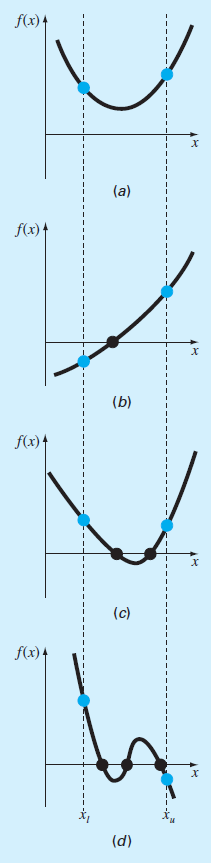
\includegraphics[width=.65\linewidth]{./images/fig_5_1}
        \captionof{figure}{Illustration of a number of general ways that a root may
            occur in an interval prescribed by a lower bound $x_l$ and
            an upper bound $x_u$. Parts (a) and (c) indicate that if both
            $f(x_l)$ and $f(x_u)$ have the same sign, either there will
            be no roots or there will be an even number of roots
            within the interval. Parts (b) and (d) indicate that if the
            function has different signs at the end points, there will
            be an odd number of roots in the interval.}
    \end{minipage}
    \hfill
    \begin{minipage}[b]{.48\textwidth}
        \centering
        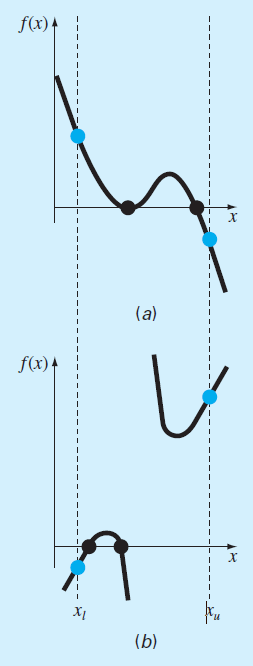
\includegraphics[width=.65\linewidth]{./images/fig_5_2}
        \captionof{figure}{Illustration of some exceptions to the general cases
            depicted in Fig. 5.1. (a) Multiple roots that occur when
            the function is tangential to the $x$ axis. For this case,
            although the end points are of opposite signs, there are
            an even number of axis interceptions for the interval.
            (b) Discontinuous functions where end points of opposite
            sign bracket an even number of roots. Special strategies
            are required for determining the roots for these cases.}
    \end{minipage}
\end{figure}
\newpage

For well-posed problems, the bracketing methods always work but converge slowly
(i.e., they typically take more iterations to home in on the answer). In contrast, the open
methods do not always work (i.e., they can diverge), but when they do they usually converge
quicker.

In both cases, initial guesses are required. These may naturally arise from the physical
context you are analyzing. However, in other cases, good initial guesses may not be obvious.
In such cases, automated approaches to obtain guesses would be useful. The following
section describes one such approach, the incremental search.

\subsection{Incremental Search}
\noindent When applying the graphical technique in Example 5.1, you observed that $f(x)$ changed
sign on opposite sides of the root. In general, if $f(x)$ is real and continuous in the interval
from $x_l$ to $x_u$ and $f(x_l)$ and $f(x_u)$ have opposite signs, that is, \\

$f(x_l)f(x_u) < 0$
\hfill (5.3)\\

\noindent then there is at least one real root between $x_l$ and $x_u$ .

\emph{Incremental search} methods capitalize on this observation by locating an interval
where the function changes sign. A potential problem with an incremental search is the
choice of the increment length. If the length is too small, the search can be very time consuming.
On the other hand, if the length is too great, there is a possibility that closely
spaced roots might be missed (Fig. 5.3). The problem is compounded by the possible existence
of multiple roots.

An M-file can be developed\footnote{This function is a modified version of an M-file originally
presented by Recktenwald (2000).} that implements an incremental search to locate the roots
of a function \texttt{func} within the range from \texttt{xmin} to \texttt{xmax} (Fig. 5.4). An optional argument
ns allows the user to specify the number of intervals within the range. If ns is omitted, it
is automatically set to 50. A \texttt{for} loop is used to step through each interval. In the event that
a sign change occurs, the upper and lower bounds are stored in an array \texttt{xb}.\\

\bigskip
\begin{figure}[h]
    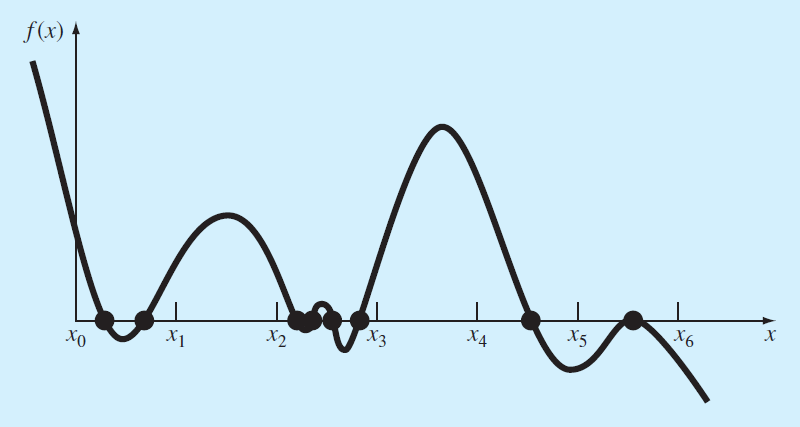
\includegraphics[width=0.8\linewidth]{./images/fig_5_3}
    \caption{Cases where roots could be missed because the incremental length of the search procedure is
    too large. Note that the last root on the right is multiple and would be missed regardless of the
    increment length.}
\end{figure}
\newpage

\begin{figure}[h]
    \begin{lstlisting}[numbers=none]
 function xb = incsearch(func,xmin,xmax,ns)
 % incsearch: incremental search root locator
 %    xb = incsearch(func,xmin,xmax,ns):
 %       finds brackets of x that contain sign changes
 %       of a function on an interval
 % input:
 %    func = name of function
 %    xmin, xmax = endpoints of interval
 %    ns = number of subintervals (default = 50)
 % output:
 %    xb(k,1) is the lower bound of the kth sign change
 %    xb(k,2) is the upper bound of the kth sign change
 %    If no brackets found, xb = [].
 if nargin < 3, error('at least 3 arguments required'), end
 if nargin < 4, ns = 50; end %if ns blank set to 50
 % Incremental search
 x = linspace(xmin,xmax,ns);
 f = func(x);
 nb = 0; xb = []; %xb is null unless sign change detected
 for k = 1:length(x)-1
    if sign(f(k)) ~= sign(f(k+1)) %check for sign change
       nb = nb + 1;
       xb(nb,1) = x(k);
       xb(nb,2) = x(k+1);
    end
 end
 if isempty(xb) %display that no brackets were found
    disp('no brackets found')
    disp('check interval or increase ns')
 else
    disp('number of brackets:') %display number of brackets
    disp(nb)
 end
    \end{lstlisting}
    \caption{An M-file to implement an incremental search.}
\end{figure}

\begin{example} Incremental Search\\

    \noindent\textbf{Problem Statement.}\quad Use the M-file incsearch (Fig. 5.4) to identify brackets within the
    interval [3, 6] for the function:\\

    $f(x) = sin(10x)+cos(3x)$
    \hfill (5.4)\\

    \noindent\textbf{Solution.}\quad The MATLAB session using the default number of intervals (50) is\\

    \noindent\texttt{>> incsearch(@(x) sin(10*x)+cos(3*x),3,6)\\
    number of brackets:\\
    \indent 5\\
    \noindent ans =\\
    \indent 3.2449 \indent 3.3061\\
    \indent 3.3061 \indent 3.3061\\
    \indent 3.7347 \indent 3.7959\\
    \indent 4.6531 \indent 4.7143\\
    \indent 5.6327 \indent 5.6939\\}

    \noindent A plot of Eq. (5.4) along with the root locations is shown here.
    \newpage

    \begin{figure}[h]
        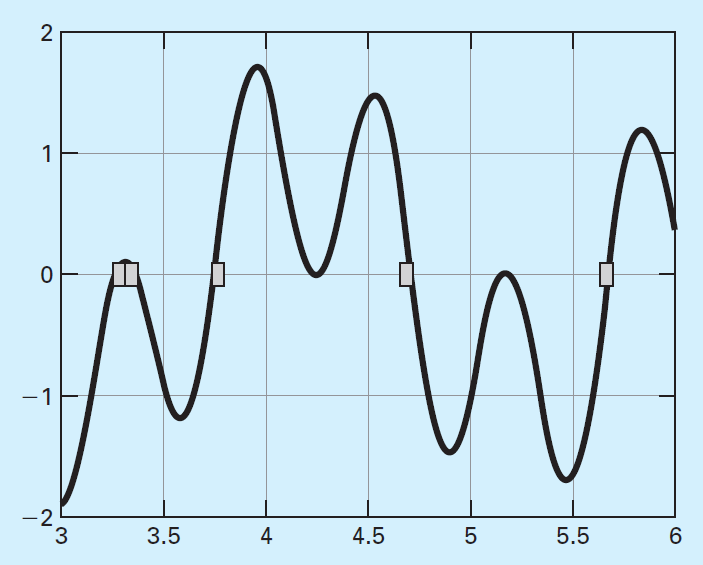
\includegraphics[width=0.65\linewidth]{./images/example_5_2_1}
    \end{figure}

    \noindent Although five sign changes are detected, because the subintervals are too wide, the function
    misses possible roots at $x\cong 4.25$ and $5.2$. These possible roots look like they might be
    double roots. However, by using the zoom in tool, it is clear that each represents two real
    roots that are very close together. The function can be run again with more subintervals
    with the result that all nine sign changes are located\\

    \texttt{>> incsearch(@(x) sin(10*x)+cos(3*x),3,6,100)\\
    number of brackets:\\
    \indent 9\\
    ans =\\
        \indent 3.2424 \indent 3.2727\\
        \indent 3.3636 \indent 3.3939\\
        \indent 3.7273 \indent 3.7576\\
        \indent 4.2121 \indent 4.2424\\
        \indent 4.2424 \indent 4.2727\\
        \indent 4.6970 \indent 4.7273\\
        \indent 5.1515 \indent 5.1818\\
        \indent 5.1818 \indent 5.2121\\
        \indent 5.6667 \indent 5.6970\\}

    \begin{figure}[h]
        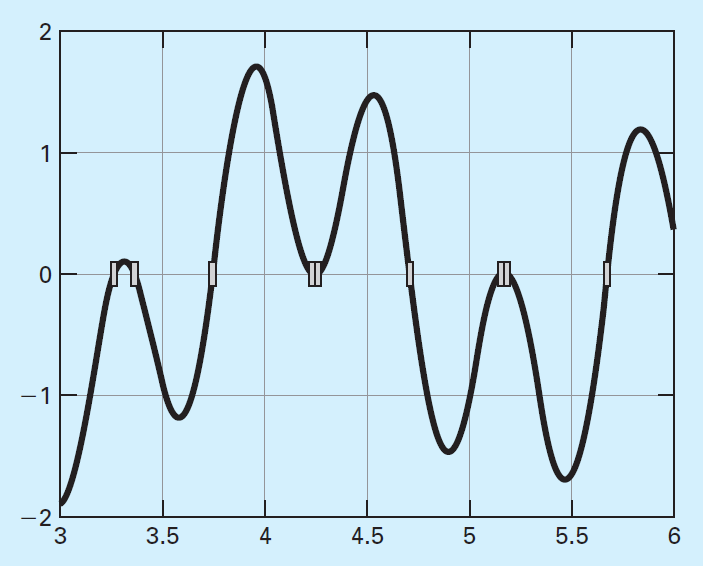
\includegraphics[width=0.65\linewidth]{./images/example_5_2_2}
    \end{figure}

    The foregoing example illustrates that brute-force methods such as incremental search
    are not foolproof. You would be wise to supplement such automatic techniques with any
    other information that provides insight into the location of the roots. Such information can
    be found by plotting the function and through understanding the physical problem from
    which the equation originated.
\end{example}

\section[BISECTION]{BISECTION}
\noindent 
The \emph{bisection method} is a variation of the incremental search method in which the interval
is always divided in half. If a function changes sign over an interval, the function value at
the midpoint is evaluated. The location of the root is then determined as lying within the
subinterval where the sign change occurs. The subinterval then becomes the interval for
the next iteration. The process is repeated until the root is known to the required precision.
A graphical depiction of the method is provided in Fig. 5.5. The following example goes
through the actual computations involved in the method.

\begin{example} The Bisection Method\\

    \noindent\textbf{Problem Statement.}\quad Use bisection to solve the same problem approached graphically in
    Example 5.1.\\

    \begin{figure}[h]
        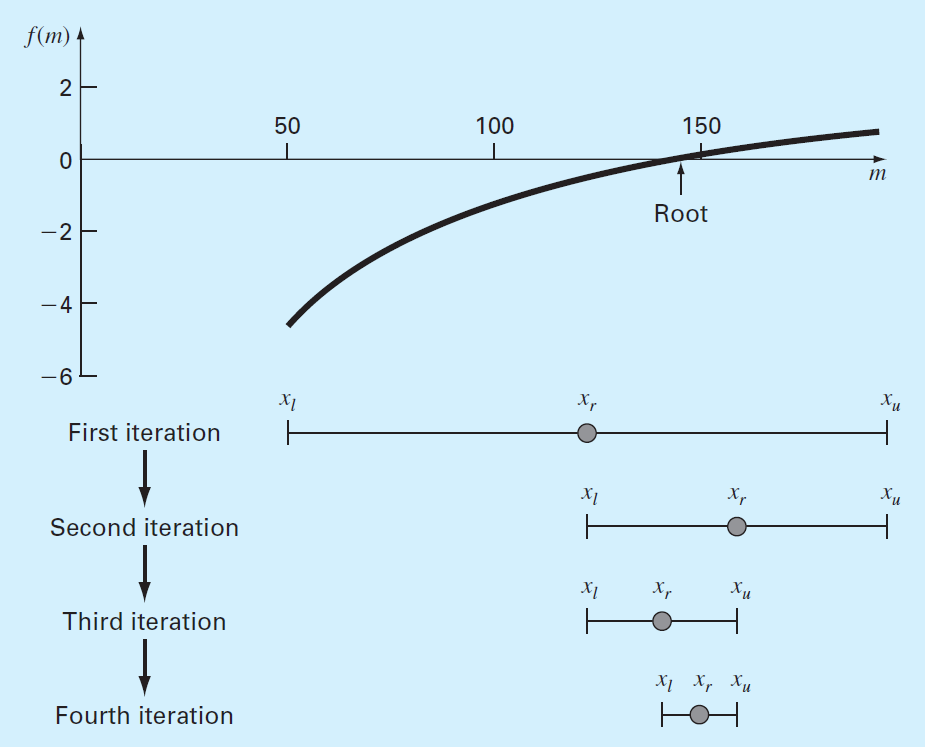
\includegraphics[width=0.7\linewidth]{./images/fig_5_5}
        \caption{A graphical depiction of the bisection method. This plot corresponds to the first four iterations
        from Example 5.3.}
    \end{figure}

    \noindent\textbf{Solution.} \quad The first step in bisection is to guess two values of the unknown (in the present
    problem, $m$) that give values for $f (m)$ with different signs. From the graphical solution in 
    Example 5.1, we can see that the function changes sign between values of 50 and 200. The
    plot obviously suggests better initial guesses, say 140 and 150, but for illustrative purposes
    let's assume we don't have the benefit of the plot and have made conservative guesses.
    Therefore, the initial estimate of the root $x_r$ lies at the midpoint of the interval\\

    $x_r = \dfrac{50+200}{2}=125$\\

    \noindent Note that the exact value of the root is 142.7376. This means that the value of 125 calculated
    here has a true percent relative error of\\

    $\left\lvert \epsilon_t \right\rvert = \left\lvert \dfrac{142.7376-125}{142.7376} \right\rvert\times 100\% = 12.43\%$\\

    \noindent Next we compute the product of the function value at the lower bound and at the midpoint:\\

    $f(50)f(125) = -4.579(-0.409)=1.871$\\

    \noindent which is greater than zero, and hence no sign change occurs between the lower bound and
    the midpoint. Consequently, the root must be located in the upper interval between 125 and
    200. Therefore, we create a new interval by redefining the lower bound as 125.

    At this point, the new interval extends from $x_l = 125$ to $x_u = 200$. Arevised root estimate
    can then be calculated as\\

    $x_r = \dfrac{125+200}{2}=162.5$\\

    \noindent which represents a true percent error of $\left\lvert \epsilon_t \right\rvert = 13.85\%$. The process can be repeated to obtain
    refined estimates. For example,\\

    $f(125)f(162.5) = -0.409(0.359)=-0.147$\\

    \noindent Therefore, the root is now in the lower interval between 125 and 162.5. The upper bound
    is redefined as 162.5, and the root estimate for the third iteration is calculated as\\

    $x_r = \dfrac{125+162.5}{2} = 143.75$\\

    \noindent which represents a percent relative error of $\epsilon_t = 0.709\%$. The method can be repeated until
    the result is accurate enough to satisfy your needs.\\
\end{example}

We ended Example 5.3 with the statement that the method could be continued to obtain
a refined estimate of the root. We must now develop an objective criterion for deciding when
to terminate the method.

An initial suggestion might be to end the calculation when the error falls below some
prespecified level. For instance, in Example 5.3, the true relative error dropped from 12.43
to $0.709\%$ during the course of the computation. We might decide that we should terminate
when the error drops below, say, $0.5\%$. This strategy is flawed because the error estimates
in the example were based on knowledge of the true root of the function. This would not be
the case in an actual situation because there would be no point in using the method if we
already knew the root.

Therefore, we require an error estimate that is not contingent on foreknowledge of the
root. One way to do this is by estimating an approximate percent relative error as in [recall
Eq. (4.5)]\\

$\left\lvert \epsilon_a \right\rvert = \left\lvert \dfrac{x^{new}_r - x^{old}_r}{x^{new}_r} \right\rvert 100\%$
\hfill (5.5)\\

\noindent where $x^{new}_r$ is the new root for the present iteration and $x^{old}_r$ is the root 
from the previous iteration. When $\epsilon_a$ becomes less than a prespecified stopping criterion 
$\epsilon_s$, the computation is terminated.\\

\begin{example} Error Estimates for Bisection\\
    
    \noindent\textbf{Problem Statement.}\quad Continue Example 5.3 until the approximate error falls below a
    stopping criterion of $\epsilon_s = 0.5\%$. Use Eq. (5.5) to compute the errors.\\

    \noindent\textbf{Solution.} The results of the first two iterations for Example 5.3 were 125 and 162.5. Substituting
    these values into Eq. (5.5) yields\\

    $\left\lvert \epsilon_a \right\rvert = \left\lvert \dfrac{162.5-125}{162.5} \right\rvert 100\% = 23.08\%$\\

    \noindent Recall that the true percent relative error for the root estimate of 162.5 was $13.85\%$. Therefore,
    $\left\lvert \epsilon_a \right\rvert$ is greater than $\epsilon_t$. This behavior is manifested for the other iterations:\\

    \begin{figure}[h]
        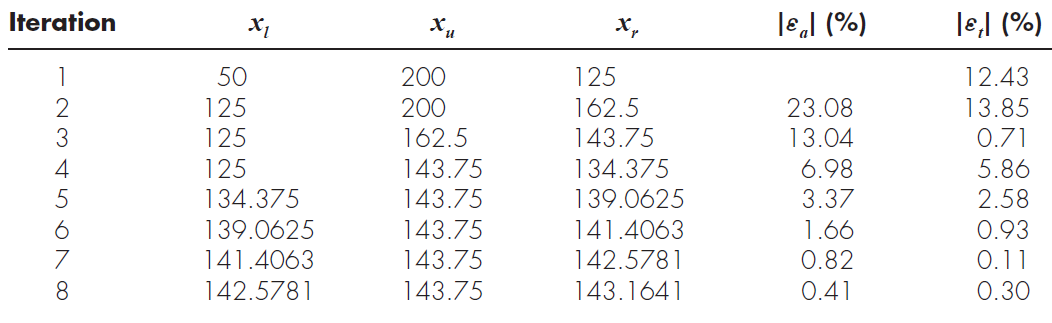
\includegraphics[width=0.75\linewidth]{./images/example_5_4_1}
    \end{figure}
    \vspace{1cm}
    
    \noindent Thus after eight iterations $\left\lvert \epsilon_a \right\rvert $ finally falls below $\epsilon_s = 0.5\%$, and the computation can be
    terminated.

    These results are summarized in Fig. 5.6. The ``ragged'' nature of the true error is due
    to the fact that, for bisection, the true root can lie anywhere within the bracketing interval.
    The true and approximate errors are far apart when the interval happens to be centered
    on the true root. They are close when the true root falls at either end of the interval.

    \begin{figure}[h]
        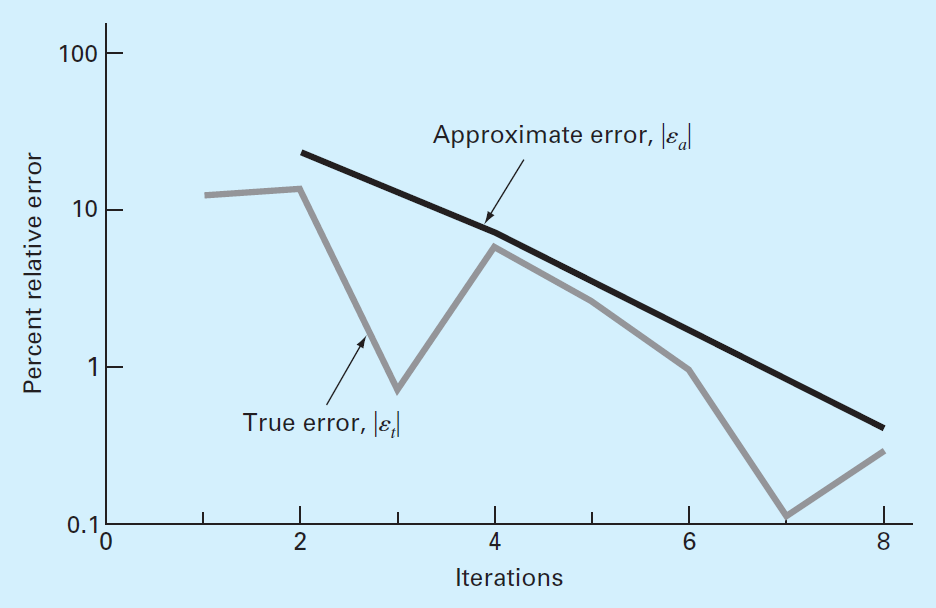
\includegraphics[width=0.8\linewidth]{./images/fig_5_6}
        \caption{Errors for the bisection method. True and approximate errors are plotted versus the number
        of iterations.}
    \end{figure}    
\end{example}

Although the approximate error does not provide an exact estimate of the true error,
Fig. 5.6 suggests that $\left\lvert \epsilon_a \right\rvert $ captures the general downward trend of $\epsilon_t$. In addition, the plot
exhibits the extremely attractive characteristic that $\epsilon_a$ is always greater than $\epsilon_t$. Thus,
when $\epsilon_a$ falls below $\epsilon_s$ , the computation could be terminated with confidence that the root
is known to be at least as accurate as the prespecified acceptable level.

While it is dangerous to draw general conclusions from a single example, it can be
demonstrated that $\epsilon_a$ will always be greater than $\epsilon_t$ for bisection. This is due to the fact
that each time an approximate root is located using bisection as $x_r = (x_l + x_u)/2$, we know
that the true root lies somewhere within an interval of $\Delta x = x_u - x_l$. Therefore, the root
must lie within $\pm\Delta x/2$ of our estimate. For instance, when Example 5.4 was terminated,
we could make the definitive statement that\\

$x_r = 143.1641\pm\dfrac{143.7500-142.5781}{2}=143.1641\pm 0.5859$\\

In essence, Eq. (5.5) provides an upper bound on the true error. For this bound to be
exceeded, the true root would have to fall outside the bracketing interval, which by definition
could never occur for bisection. Other root-locating techniques do not always behave
as nicely. Although bisection is generally slower than other methods, the neatness of its
error analysis is a positive feature that makes it attractive for certain engineering and
scientific applications.

Another benefit of the bisection method is that the number of iterations required to attain
an absolute error can be computed \emph{a priori}---that is, before starting the computation.
This can be seen by recognizing that before starting the technique, the absolute error is\\

$E^0_a = x^0_u-x^0_l = \Delta x^0$\\

\noindent where the superscript designates the iteration. Hence, before starting the method we are at
the ``zero iteration''. After the first iteration, the error becomes\\

$E^1_a = \dfrac{\Delta x^0}{2}$\\

\noindent Because each succeeding iteration halves the error, a general formula relating the error and
the number of iterations $n$ is\\

$E^n_a = \dfrac{\Delta x^0}{2^n}$\\

\noindent If $E_{a,d}$ is the desired error, this equation can be solved for\footnote{MATLAB provides the \texttt{log2} function to evaluate the base-2 logarithm directly. If the pocket calculator or
computer language you are using does not include the base-2 logarithm as an intrinsic function, this equation
shows a handy way to compute it. In general, $log_b(x) = log(x)/log(b)$.}\\

$n = \dfrac{log(\Delta x^0/E_{a,d})}{log2}=log_2\Big(\dfrac{\Delta x^0}{E_{a,d}}\Big)$
\hfill (5.6)\\

Let's test the formula. For Example 5.4, the initial interval was $\Delta x = 200-50 = 150$.
After eight iterations, the absolute error was\\

$E_a = \dfrac{\left\lvert 143.7500 - 142.5781 \right\rvert}{2} = 0.5859$\\

\noindent We can substitute these values into Eq. (5.6) to give\\

$n = log_2(150/0.5859) = 8$\\

\noindent Thus, if we knew beforehand that an error of less than 0.5859 was acceptable, the formula
tells us that eight iterations would yield the desired result.

Although we have emphasized the use of relative errors for obvious reasons, there will
be cases where (usually through knowledge of the problem context) you will be able to
specify an absolute error. For these cases, bisection along with Eq. (5.6) can provide a useful
root-location algorithm.\\

\subsection{\textbf{MATLAB M-file}: bisect}
\noindent An M-file to implement bisection is displayed in Fig. 5.7. It is passed the function (\texttt{func})
along with lower (\texttt{xl}) and upper (\texttt{xu}) guesses. In addition, an optional stopping criterion (\texttt{es})
and maximum iterations (\texttt{maxit}) can be entered. The function first checks whether there
are sufficient arguments and if the initial guesses bracket a sign change. If not, an error
message is displayed and the function is terminated. It also assigns default values if \texttt{maxit}
and \texttt{es} are not supplied. Then a \texttt{while...break} loop is employed to implement the
bisection algorithm until the approximate error falls below es or the iterations exceed
\texttt{maxit}.

We can employ this function to solve the problem posed at the beginning of the chapter.
Recall that you need to determine the mass at which a bungee jumper's free-fall velocity
exceeds 36 m/s after 4 s of free fall given a drag coefficient of 0.25 kg/m. Thus, you have to
find the root of\\

$f(m) = \sqrt{\dfrac{9.81m}{0.25}}$tanh$\Big(\sqrt{\dfrac{9.81(0.25)}{m}}4 \Big)-36$\\

\noindent In Example 5.1 we generated a plot of this function versus mass and estimated that the root
fell between 140 and 150 kg. The \texttt{bisect} function from Fig. 5.7 can be used to determine
the root as\\

\texttt{>> fm=@(m) sqrt(9.81*m/0.25)*tanh(sqrt(9.81*0.25/m)*4)-36;\\
\indent >> [mass fx ea iter]=bisect(fm,40,200)\\
\indent mass =\\
\indent\indent 142.74\\
\indent fx =\\
\indent\indent 4.6089e-007\\
\indent ea =\\
\indent\indent 5.345e-005\\
\indent iter =\\
\indent\indent 21\\}

\noindent Thus, a result of $m$ = 142.74 kg is obtained after 21 iterations with an approximate relative
error of $\epsilon_a = 0.00005345\%$, and a function value close to zero.

\begin{figure}[h]
    \begin{lstlisting}[numbers=none]
 function [root,fx,ea,iter]=bisect(func,xl,xu,es,maxit,varargin)
 % bisect: root location zeroes
 %    [root,fx,ea,iter]=bisect(func,xl,xu,es,maxit,p1,p2,...):
 %       uses bisection method to find the root of func
 % input:
 %    func = name of function
 %    xl, xu = lower and upper guesses
 %    es = desired relative error (default = 0.0001%)
 %    maxit = maximum allowable iterations (default = 50)
 %    p1,p2,... = additional parameters used by func
 % output:
 %    root = real root
 %    fx = function value at root
 %    ea = approximate relative error (%)
 %    iter = number of iterations
 if nargin<3,error('at least 3 input arguments required'),end
 test = func(xl,varargin{:})*func(xu,varargin{:});
 if test>0,error('no sign change'),end
 if nargin<4|isempty(es), es=0.0001;end
 if nargin<5|isempty(maxit), maxit=50;end
 iter = 0; xr = xl; ea = 100;
 while (1)
    xrold = xr;
    xr = (xl + xu)/2;
    iter = iter + 1;
    if xr ~= 0,ea = abs((xr - xrold)/xr) * 100;end
    test = func(xl,varargin{:})*func(xr,varargin{:});
    if test < 0
       xu = xr;
    elseif test > 0
       xl = xr;
    else
       ea = 0;
    end
    if ea <= es | iter >= maxit,break,end
 end
 root = xr; fx = func(xr, varargin{:});
    \end{lstlisting}
    \caption{An M-file to implement the bisection method.}
\end{figure}
\vspace{1.5 cm}

\newpage

\section[FALSE POSITIVE]{FALSE POSITIVE}
\noindent \emph{False position} (also called the linear interpolation method) is another well-known bracketing
method. It is very similar to bisection with the exception that it uses a different strategy
to come up with its new root estimate. Rather than bisecting the interval, it locates the root
by joining $f (x_l )$ and $f (x_u)$ with a straight line (Fig. 5.8). The intersection of this line with
the $x$ axis represents an improved estimate of the root. Thus, the shape of the function influences
the new root estimate. Using similar triangles, the intersection of the straight line
with the $x$ axis can be estimated as (see Chapra and Canale, 2010, for details),

$x_r = x_u - \dfrac{f(x_u)(x_l-x_u)}{f(x_l)-f(x_u)}$
\hfill (5.7)\\

This is the \emph{false-position formula}. The value of $x_r$ computed with Eq. (5.7) then replaces
whichever of the two initial guesses, $x_l$ or $x_u$, yields a function value with the same
sign as $f (x_r )$. In this way the values of $x_l$ and $x_u$ always bracket the true root. The process
is repeated until the root is estimated adequately. The algorithm is identical to the one for
bisection (Fig. 5.7) with the exception that Eq. (5.7) is used.\\
\newpage

\begin{figure}[h]
    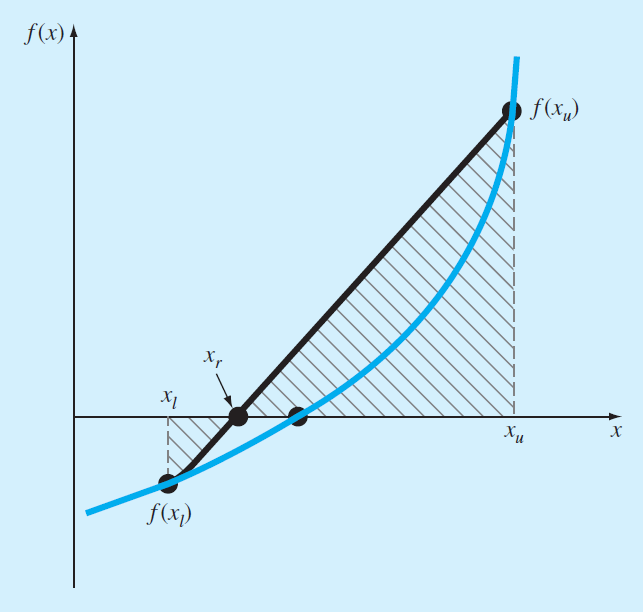
\includegraphics[width=0.65\linewidth]{./images/fig_5_8}
    \caption{False position.}
\end{figure}

\begin{example} The False-Position Method\\

    \noindent\textbf{Problem Statement.}\quad Use false position to solve the same problem approached graphically
    and with bisection in Examples 5.1 and 5.3.\\

    \noindent\textbf{Solution.}\quad As in Example 5.3, initiate the computation with guesses of $x_l = 50$ and
    $x_u = 200$.\\

    \noindent First iteration:\\

    $x_l = 50\text{ }$ \indent$f(x_l)$\\

    $x_u=200$\indent$f(x_u)=0.860291$\\

    $x_r=200-\dfrac{0.860291(50 - 200)}{-4.579387 - 0.860291}=176.2773$\\

    \noindent which has a true relative error of $23.5\%$.\\

    \noindent Second iteration:\\

    $f(x_l)f(x_r)=-2.592732$\\

    \noindent Therefore, the root lies in the first subinterval, and $x_r$ becomes the upper limit for the next
    iteration, $x_u = 176.2773$.\\

    $x_l=50$\hspace{22.5mm}$f(x_l) = -4.579387$\\

    $x_u=176.2773$\indent$f(x_u)=0.566174$\\

    $x_r=176.2773-\dfrac{0.566174(50 - 176.2773)}{-4.579387 - 0.566174}=162.3828$\\

    \noindent which has true and approximate relative errors of $13.76\%$ and $8.56\%$, respectively. Additional
    iterations can be performed to refine the estimates of the root.
\end{example}

Although false position often performs better than bisection, there are other cases
where it does not. As in the following example, there are certain cases where bisection
yields superior results.\\

\begin{example} A Case Where Bisection Is Preferable to False Position\\

    \noindent\textbf{Problem Statement.}\quad  Use bisection and false position to locate the root of\\

    $f(x)=x^{10}-1$\\

    \noindent between $x = 0$ and 1.3.\\

    \noindent\textbf{Solution.} Using bisection, the results can be summarized as

    \begin{figure}[h]
        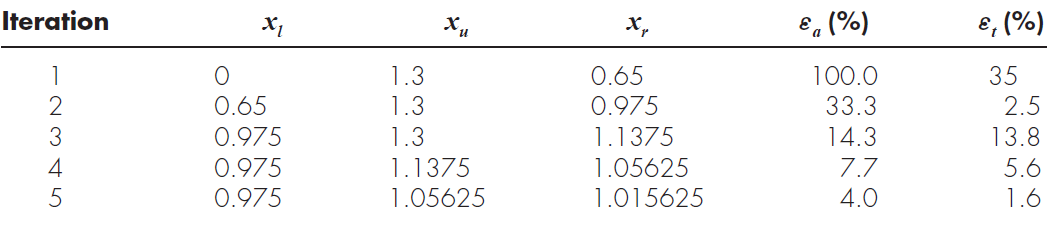
\includegraphics[width=0.8\linewidth]{./images/example_5_6_1}
    \end{figure}

    \noindent Thus, after five iterations, the true error is reduced to less than $2\%$. For false position, a
    very different outcome is obtained:\\

    \begin{figure}[h]
        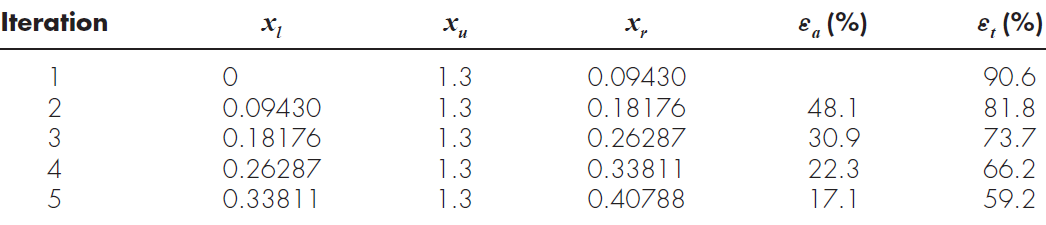
\includegraphics[width=0.8\linewidth]{./images/example_5_6_2}
    \end{figure}

    After five iterations, the true error has only been reduced to about $59\%$. Insight into
    these results can be gained by examining a plot of the function. As in Fig. 5.9, the curve
    violates the premise on which false position was based---that is, if $f (x_l )$ is much closer to
    zero than $f (x_u)$, then the root should be much closer to $x_l$ than to $x_u$ (recall Fig. 5.8). Because
    of the shape of the present function, the opposite is true.\\

    \begin{figure}[h]
        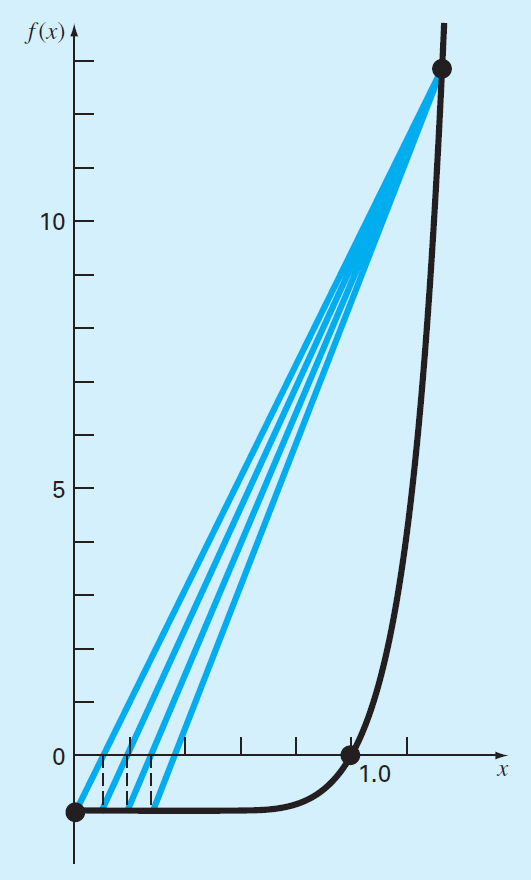
\includegraphics[width=0.35\linewidth]{./images/fig_5_9}
        \caption{Plot of $f (x) = x^{10} - 1$, illustrating slow convergence of the false-position method.}
    \end{figure}
\end{example}

The foregoing example illustrates that blanket generalizations regarding rootlocation
methods are usually not possible. Although a method such as false position is
often superior to bisection, there are invariably cases that violate this general conclusion.
Therefore, in addition to using Eq. (5.5), the results should always be checked by substituting
the root estimate into the original equation and determining whether the result is
close to zero.

The example also illustrates a major weakness of the false-position method: its onesidedness.
That is, as iterations are proceeding, one of the bracketing points will tend to
stay fixed. This can lead to poor convergence, particularly for functions with significant
curvature. Possible remedies for this shortcoming are available elsewhere (Chapra and
Canale, 2010).\\
\bigskip

\section[CASE STUDY: GREENHOUSE GASES AND RAINWATER]{CASE STUDY: GREENHOUSE GASES AND RAINWATER}
\noindent\textbf{Background.}\quad It is well documented that the atmospheric levels of several so-called
``greenhouse'' gases have been increasing over the past 50 years. For example, Fig. 5.10
shows data for the partial pressure of carbon dioxide $(CO_2)$ collected at Mauna Loa, Hawaii
from 1958 through 2008. The trend in these data can be nicely fit with a quadratic polynomial,
\footnote{In Part Four, we will learn how to determine such polynomials.}\\

$p_{CO_2} = 0.012226(t - 1983)^2 + 1.418542(t - 1983) + 342.38309$\\

\noindent where $p_{CO_2} = CO_2$ partial pressure (ppm). These data indicate that levels have increased a
little over $22\%$ over the period from 315 to 386 ppm.
One question that we can address is how this trend is affecting the pH of rainwater.
Outside of urban and industrial areas, it is well documented that carbon dioxide is the primary
determinant of the pH of the rain. pH is the measure of the activity of hydrogen ions
and, therefore, its acidity or alkalinity. For dilute aqueous solutions, it can be computed as\\

$pH=-log_{10}[H^+]$
\hfill (5.8)\\

\noindent where $[H^+]$ is the molar concentration of hydrogen ions.\\
\noindent The following five equations govern the chemistry of rainwater:\\

$K_1 = 10^6 \dfrac{[H^+][HCO^-_3]}{K_H p_{CO_2}}$
\hfill (5.9)\\

\begin{figure}[h]
    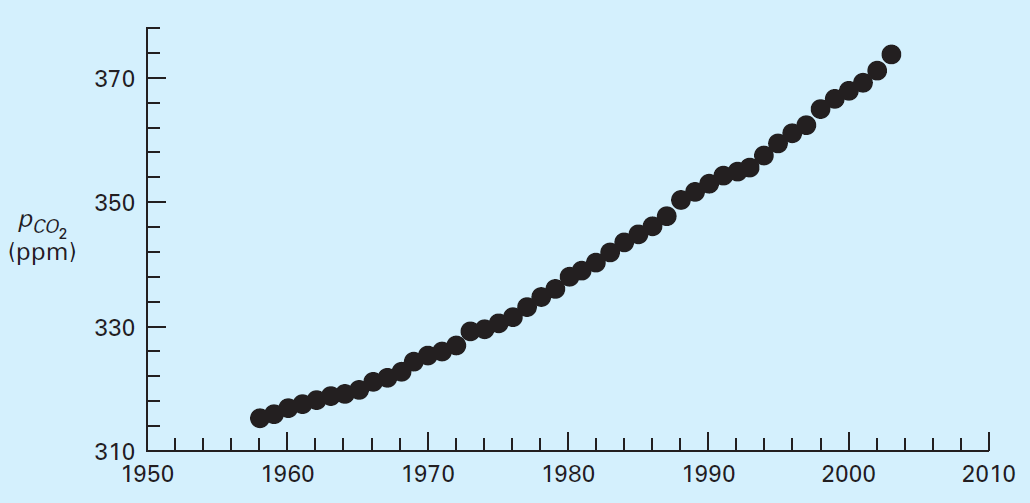
\includegraphics[width=0.7\linewidth]{./images/fig_5_10}
    \caption{Average annual partial pressures of atmospheric carbon dioxide (ppm) measured at Mauna Loa,
    Hawaii.}
\end{figure}

$K_2=\dfrac{[H^+][CO^{-2}_3]}{HCO^-_3}$
\hfill (5.10)\\

$K_w = [H^+][OH^-]$
\hfill (5.11)\\

$c_T=\dfrac{K_H p_{CO_2}}{10^6}+[HCO^-_3]+[CO^{-2}_3]$
\hfill (5.12)\\

$0=[HCO^-_3]+2[CO^{-2}_3]+[OH^-]-[H^+]$
\hfill (5.13)\\

\noindent where $K_H$ = Henry's constant, and $K_1$, $K_2$, and $K_w$ are equilibrium coefficients. The five
unknowns are $c_T$ = total inorganic carbon, $[HCO^-_3 ]$ = bicarbonate, $[CO^{-2}_3 ]$ = carbonate,
$[H^+]$ = hydrogen ion, and $[OH^-]$ = hydroxyl ion. Notice how the partial pressure of $CO_2$
shows up in Eqs. (5.9) and (5.12).

Use these equations to compute the pH of rainwater given that $K_H =10^{-1.46}$,
 $K_1 = 10^{-6.3}$, $K_2 = 10^{-10.3}$, and $K_w = 10^{-14}$. Compare the results in 1958 when
the $p_{CO_2}$ was 315 and in 2008 when it was 386 ppm. When selecting a numerical method
for your computation, consider the following:

\begin{itemize}
    \item You know with certainty that the pH of rain in pristine areas always falls between 2
    and 12.
    \item You also know that pH can only be measured to two places of decimal precision.
\end{itemize}

\noindent\textbf{Solution.}\quad There are a variety of ways to solve this system of five equations. One way
is to eliminate unknowns by combining them to produce a single function that only depends
on $[H^+]$. To do this, first solve Eqs. (5.9) and (5.10) for\\

$[HCO^-_3]=\dfrac{K_1}{10^6[H^+]}K_H p_{CO_2}$
\hfill (5.14)\\

$[CO^{-2}_3]=\dfrac{K_2[HCO^-_3]}{[H^+]}$
\hfill (5.15)\\

\noindent Substitute Eq. (5.14) into (5.15)\\

$[CO^{-2}_3]=\dfrac{K_2K_1}{10^6[H^+]^2}K_Hp_{CO_2}$
\hfill (5.16)\\

\noindent Equations (5.14) and (5.16) can be substituted along with Eq. (5.11) into Eq. (5.13) to give\\

$0=\dfrac{K_1}{10^6[H^+]}K_H p_{CO_2} + 2\dfrac{K_2K_1}{10^6[H^+]^2}K_Hp_{CO_2} + \dfrac{K_w}{[H^+]}-[H^+]$
\hfill (5.17)\\

\noindent Although it might not be immediately apparent, this result is a third-order polynomial in
$[H^+]$. Thus, its root can be used to compute the pH of the rainwater.

Now we must decide which numerical method to employ to obtain the solution. There
are two reasons why bisection would be a good choice. First, the fact that the pH always
falls within the range from 2 to 12, provides us with two good initial guesses. Second, because
the pH can only be measured to two decimal places of precision, we will be satisfied
with an absolute error of $E_{a,d} = \pm0.005$. Remember that given an initial bracket and the
desired error, we can compute the number of iteration \emph{a priori}. Substituting the present values
into Eq. (5.6) gives\\

\texttt{>> dx=12-2;\\
\indent >> Ead=0.005;\\
\indent >> n=log2(dx/Ead)\\
\indent n =\\
\indent\indent 10.9658\\}

\noindent Eleven iterations of bisection will produce the desired precision.\\
Before implementing bisection, we must first express Eq. (5.17) as a function. Because
it is relatively complicated, we will store it as an M-file:\\

\texttt{function f = fpH(pH,pCO2)\\
\indent K1=10\textasciicircum -6.3;K2=10\textasciicircum-10.3;Kw=10\textasciicircum-14;\\
\indent KH=10\textasciicircum-1.46;\\
\indent H=10\textasciicircum-pH;\\
\indent f=K1/(1e6*H)*KH*pCO2+2*K2*K1/(1e6*H)*KH*pCO2+Kw/H-H;\\}

We can then use the M-file from Fig. 5.7 to obtain the solution. Notice how we have
set the value of the desired relative error $(\epsilon_a = 1 \times 10^-8)$ at a very low level so that the iteration
limit (\texttt{maxit}) is reached first so that exactly 11 iterations are implemented\\

\texttt{>> [pH1958 fx ea iter]=bisect(@fpH,2,12,1e-8,11,315)\\
\indent pH1958 =\\
\indent\indent 5.6279\\
\indent fx =\\
\indent\indent -2.7163e-008\\
\indent ea =\\
\indent\indent 0.08676\\
\indent iter =\\
\indent\indent 11\\}

\noindent Thus, the pH is computed as 5.6279 with a relative error of $0.0868\%$. We can be confident
that the rounded result of 5.63 is correct to two decimal places. This can be verified by performing
another run with more iterations. For example, setting \texttt{maxit} to 50 yields\\

\texttt{>> [pH1958 fx ea iter] = bisect(@fpH,2,12,1e-8,50,315)\\
\indent pH1958 =\\
\indent\indent 5.6304\\
\indent fx =\\
\indent\indent 1.615e-015\\
\indent ea =\\
\indent\indent 5.169e-009\\
\indent iter =\\
\indent 35\\}

\noindent For 2008, the result is\\

\texttt{>> [pH2008 ea iter]=bisect(@fpH,2,12,1e-8,50,386)\\
\indent pH2008 =\\
\indent\indent 5.5864\\
\indent fx =\\
\indent\indent 3.2926e-015\\
\indent ea =\\
\indent\indent 5.2098e-009\\
\indent iter =\\
\indent\indent 35\\}

Interestingly, the results indicate that the $22.5\%$ rise in atmospheric $CO_2$ levels has
produced only a $0.78\%$ drop in pH. Although this is certainly true, remember that the pH
represents a logarithmic scale as defined by Eq. (5.8). Consequently, a unit drop in pH represents
an order-of-magnitude (i.e., a 10-fold) increase in the hydrogen ion. The concentration
can be computed as$ [H^+] = 10^{-pH}$ and its percent change can be calculated as.\\

\texttt{>> ((10\textasciicircum-pH2008-10\textasciicircum-pH1958)/10\textasciicircum-pH1958)*100\\
\indent ans =\\
\indent\indent 10.6791\\}

\noindent Therefore, the hydrogen ion concentration has increased about $10.7\%$.

There is quite a lot of controversy related to the meaning of the greenhouse gas trends.
Most of this debate focuses on whether the increases are contributing to global warming.
However, regardless of the ultimate implications, it is sobering to realize that something as
large as our atmosphere has changed so much over a relatively short time period. This case
study illustrates how numerical methods and MATLAB can be employed to analyze and interpret
such trends. Over the coming years, engineers and scientists can hopefully use such
tools to gain increased understanding of such phenomena and help rationalize the debate
over their ramifications.\\
\bigskip

\noindent\textbf{PROBLEMS}
\begin{multicols}{2}
    \noindent\textbf{5.1} Use bisection to determine the drag coefficient needed
    so that an 80-kg bungee jumper has a velocity of 36 m/s after
    4 s of free fall. Note: The acceleration of gravity is $9.81 m/s^2$.
    Start with initial guesses of $x_l = 0.1$ and $x_u = 0.2$ and iterate
    until the approximate relative error falls below $2\%$.\\

    \noindent\textbf{5.2} Develop your own M-file for bisection in a similar fashion
    to Fig. 5.7. However, rather than using the maximum iterations
    and Eq. (5.5), employ Eq. (5.6) as your stopping criterion. Make
    sure to round the result of Eq. (5.6) up to the next highest integer.
    Test your function by solving Prob. 5.1 using $E_{a,d} = 0.0001$.\\

    \noindent\textbf{5.3} Repeat Prob. 5.1, but use the false-position method to
    obtain your solution.\\

    \noindent\textbf{5.4} Develop an M-file for the false-position method. Test it
    by solving Prob. 5.1.\\

    \noindent\textbf{5.5 (a)} Determine the roots of $f (x) = -12 - 21x + 18x^2 - 2.75x^3$
     graphically. In addition, determine the first
    root of the function with \textbf{(b)} bisection and \textbf{(c)} false position.
    For \textbf{(b)} and \textbf{(c)} use initial guesses of $x_l = -1$ and $x_u = 0$
    and a stopping criterion of $1\%$.\\

    \noindent\textbf{5.6} Locate the first nontrivial root of $sin(x) = x^2$ where $x$ is
    in radians. Use a graphical technique and bisection with the
    initial interval from 0.5 to 1. Perform the computation until
    εa is less than $\epsilon_s = 2\%$.\\

    \noindent\textbf{5.7} Determine the positive real root of $ln(x^2) = 0.7$ \textbf{(a)}
    graphically, \textbf{(b)} using three iterations of the bisection
    method, with initial guesses of $x_l = 0.5$ and $x_u = 2$, and
    \textbf{(c)} using three iterations of the false-position method, with
    the same initial guesses as in \textbf{(b)}.\\

    \noindent\textbf{5.8} The saturation concentration of dissolved oxygen in
    freshwater can be calculated with the equation\\

    \noindent ln$o_{sf}=-139.34411+\dfrac{1.575701\times10^5}{T_a} - \dfrac{6.642308\times 10^7}{T^2_a} +
    \dfrac{1.243800\times 10^{10}}{T^3_a} - \dfrac{8.621949\times 10^{11}}{T^4_a}$\\

    \noindent where $o_{sf}$ = the saturation concentration of dissolved oxygen
    in freshwater at 1 atm $(mg L^{-1})$; and $T_a$ = absolute
    temperature (K). Remember that $T_a = T + 273.15$, where
    T = temperature (\textdegree C). According to this equation, saturation
    decreases with increasing temperature. For typical natural
    waters in temperate climates, the equation can be used to determine
    that oxygen concentration ranges from 14.621 mg/L
    at 0 \textdegree C to 6.949 mg/L at 35 \textdegree C. Given a value of oxygen concentration,
    this formula and the bisection method can be
    used to solve for temperature in \textdegree C.\\
    \textbf{(a)} If the initial guesses are set as 0 and 35 \textdegree C, how many
    bisection iterations would be required to determine temperature
    to an absolute error of 0.05 \textdegree C?\\
    \textbf{(b)} Based on \textbf{(a)}, develop and test a bisection M-file function
    to determine T as a function of a given oxygen concentration.
    Test your function for $o_{sf}$ = 8, 10 and 14 mg/L.
    Check your results.\\

    \noindent\textbf{5.9} A beam is loaded as shown in Fig. P5.9. Use the bisection
    method to solve for the position inside the beam where
    there is no moment.\\

    \noindent\textbf{5.10} Water is flowing in a trapezoidal channel at a rate of
    $Q = 20 m^3/s$. The critical depth y for such a channel must
    satisfy the equation\\

    $0=1-\dfrac{Q^2}{gA^3_c}B$\\

    \noindent where $g = 9.81 m/s^2$, $A_c$ = the cross-sectional area ($m_2$),
    and B = the width of the channel at the surface (m). For this
    case, the width and the cross-sectional area can be related to
    depth $y$ by\\

    $B=3+y$\\

    \noindent
    \begin{minipage}{\linewidth}
        \centering
        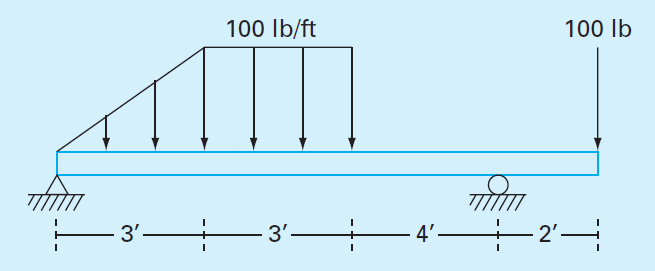
\includegraphics[width=\linewidth]{./images/problem_5_9_1}
        \captionof*{figure}{Figure P5.9}
    \end{minipage}

    \noindent and\\

    $A_c = 3y+\dfrac{y^2}{2}$\\

    \noindent Solve for the critical depth using \textbf{(a)} the graphical method,
    \textbf{(b)} bisection, and \textbf{(c)} false position. For \textbf{(b)} and \textbf{(c)} use
    initial guesses of $x_l = 0.5$ and $x_u = 2.5$, and iterate until the
    approximate error falls below $1\%$ or the number of iterations
    exceeds 10. Discuss your results.\\

    \noindent\textbf{5.11} The Michaelis-Menten model describes the kinetics of
    enzyme mediated reactions:\\

    $\dfrac{dS}{dt} = -v_m\dfrac{S}{k_s+S}$\\

    \noindent where S = substrate concentration (moles/L), $v_m$ = maximum
    uptake rate (moles/L/d), and $k_s$ = the half-saturation
    constant, which is the substrate level at which uptake is half
    of the maximum [moles/L]. If the initial substrate level at
    t = 0 is $S_0$, this differential equation can be solved for\\

    $S = S_0 - v_mt+k_s$ ln$(S_0/S)$\\

    \noindent Develop an M-file to generate a plot of S versus t for the
    case where $S_0$ = 8 moles/L, $v_m$ = 0.7 moles/L/d, and
    $k_s$ = 2.5 moles/L.\\

    \noindent\textbf{5.12} A reversible chemical reaction\\

    $2A + B \leftrightarrows C$\\

    \noindent can be characterized by the equilibrium relationship\\

    $K = \dfrac{c_c}{c^2_ac_b}$\\

    \noindent where the nomenclature $c_i$ represents the concentration of constituent
    $i$. Suppose that we define a variable $x$ as representing
    the number of moles of C that are produced. Conservation of
    mass can be used to reformulate the equilibrium relationship as

    $K = \dfrac{(c_{c,0}+x)}{(c_{a,0-2x})^2(c_{b,0}-x)}$\\

    \noindent where the subscript 0 designates the initial concentration
    of each constituent. If $K = 0.016$, $c_{a,0}= 42$, $c_{b,0} = 28$, and
    $c_{c,0}= 4$, determine the value of $x$.\\
    \textbf{(a)} Obtain the solution graphically.\\
    \textbf{(b)} On the basis of \textbf{(a)}, solve for the root with initial guesses of
    $x_l=0$ and $x_u=20$ to $\epsilon_s=0.5\%$. Choose either bisection or
    false position to obtain your solution. Justify your choice.\\

    \noindent\textbf{5.13} Figure P5.13a shows a uniform beam subject to a linearly
    increasing distributed load. The equation for the resulting
    elastic curve is (see Fig. P5.13b)\\

    $y = \dfrac{w_0}{120EIL}(-x^5+2L^2x^3-L^4x)$
    \hfill (P5.13)\\

    \noindent Use bisection to determine the point of maximum deflection
    (i.e., the value of x where $dy/dx = 0$). Then substitute this
    value into Eq. (P5.13) to determine the value of the maximum
    deflection. Use the following parameter values in your
    computation: $L = 600 cm$, $E = 50,000 kN/cm^2$, $I =
    30,000 cm^4$, and $w_0 = 2.5 kN/cm$.\\

    \noindent
    \begin{minipage}{\linewidth}
        \centering
        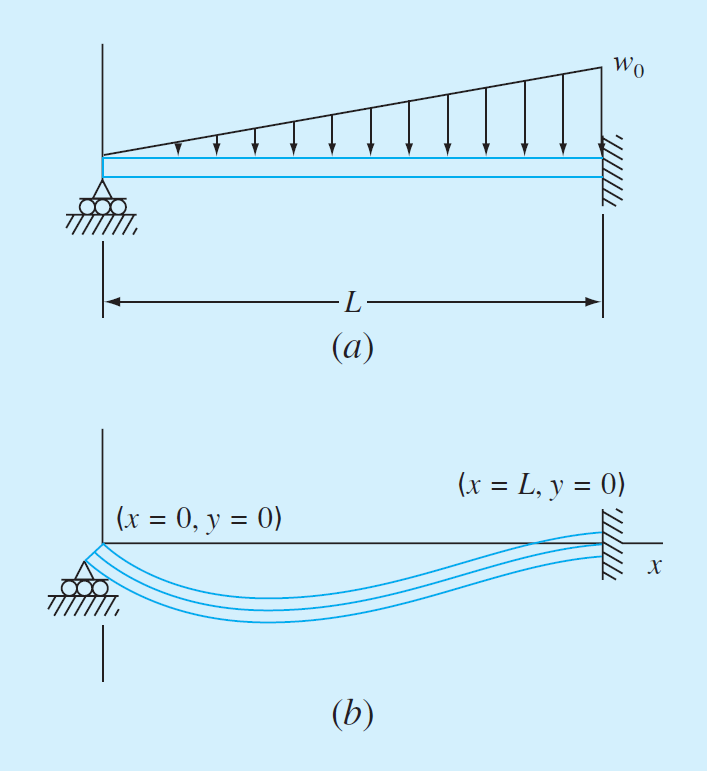
\includegraphics[width=\linewidth]{./images/problem_5_9_2}
        \captionof*{figure}{Figure P5.13}
    \end{minipage}
    \bigskip

    \noindent\textbf{5.14} You buy a \$35,000 vehicle for nothing down at \$8,500
    per year for 7 years. Use the \texttt{bisect} function from Fig. 5.7
    to determine the interest rate that you are paying. Employ
    initial guesses for the interest rate of 0.01 and 0.3 and a stopping
    criterion of 0.00005. The formula relating present
    worth $P$, annual payments $A$, number of years $n$, and interest
    rate $i$ is\\

    $A = P\dfrac{i(1+i)^n}{(i+i)^n -1}$\\

    \noindent\textbf{5.15} Many fields of engineering require accurate population
    estimates. For example, transportation engineers might find
    it necessary to determine separately the population growth
    trends of a city and adjacent suburb. The population of the
    urban area is declining with time according to\\

    $P_u(t)=P_{u,max}e^{k_ut}+P_{u,min}$\\

    \noindent while the suburban population is growing, as in\\

    $P_s(t) = \dfrac{P_{s,max}}{1+[P_{s,max}/P_0-1]e^{-k_st}}$\\

    \noindent where $P_{u,max}$, $k_u$, $P_{s,max}$, $P_0$, and $k_s$ =
    empirically derived parameters. Determine the time and corresponding values
    of $P_u(t)$ and $P_s(t)$ when the suburbs are $20\%$ larger than the city.
    The parameter values are $O_{u,max}=80,000$, $k_u=0.05/yr$, $P_{u,min}=110,000$ 
    people, $P_{s,max}=320,000$ people, $P_0=10,000$ people, and $k_s=0.09/yr$.
    To obtain your solutions, use \textbf{(a)} graphical, and \textbf{(b)} 
    false-position methods.\\

    \noindent\textbf{5.16} The resistivity $\rho$ of doped silicon is based on the
    charge $q$ on an electron, the electron density n, and the electron
    mobility $\mu$. The electron density is given in terms of
    the doping density $N$ and the intrinsic carrier density $n_i$. The
    electron mobility is described by the temperature $T$, the reference
    temperature $T_0$, and the reference mobility $μ_0$. The
    equations required to compute the resistivity are\\

    $\rho = \dfrac{1}{qn\mu}$\\

    \noindent where\\

    \noindent $n = \dfrac{1}{2}\Big(N+\sqrt{N^2+4n^2_i}\Big)$\hspace{3mm} and\hspace{3mm}
    $\mu= \mu_0 \Big(\dfrac{T}{T_0} \Big)^{-2.42}$\\

    \noindent Determine $N$, given $T_0=300$ K, $T = 1000$ K, $\mu_0=1360cm^2$ (V s)$^-1$,
    $q=1.7\times10^{-19}$ C, $n_i= 6.21\times 10^9 cm^{-3}$, and a desired $\rho = 6.5\times 10^6$ 
    V s cm/C. Employ initial guesses of $N = 0$ and $2.5\times 10^{10}$. Use \textbf{(a)} bisection
    and \textbf{(b)} the false position method.\\

    \noindent\textbf{5.17} Atotal charge $Q$ is uniformly distributed around a ringshaped
    conductor with radius $a$. A charge $q$ is located at a
    distance $x$ from the center of the ring (Fig. P5.17). The force
    exerted on the charge by the ring is given by\\

    $F = \dfrac{1}{4\pi e_0}\dfrac{qQx}{(x^2+a^2)^{3/2}}$\\

    \noindent where $e_0 = 8.9\times10^{-12}C^2/$(N m$^2$). Find the distance $x$ where the force
    is 1.25 N if $q$ and $Q$ are $2\times 10^{-5}$ C for a ring with a radius of 0.85m.\\

    \noindent
    \begin{minipage}{\linewidth}
        \centering
        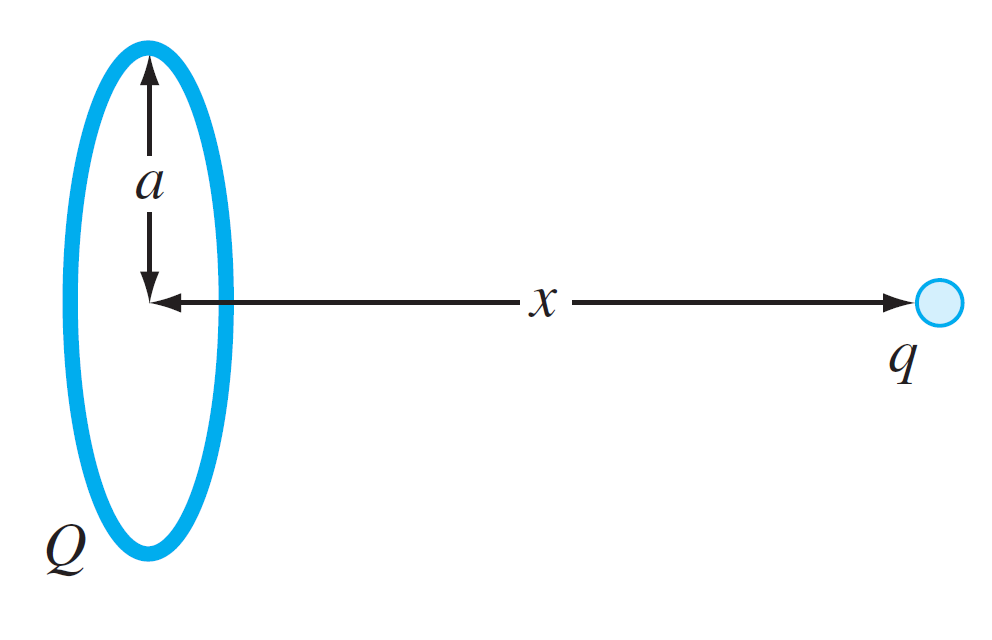
\includegraphics[width=0.65\linewidth]{./images/problem_5_9_3}
        \captionof*{figure}{Figure P5.17}
    \end{minipage}
    \bigskip

    \noindent\textbf{5.18} For fluid flow in pipes, friction is described by a dimensionless
    number, the \emph{Fanning friction factor f}. The Fanning
    friction factor is dependent on a number of parameters
    related to the size of the pipe and the fluid, which can
    all be represented by another dimensionless quantity, the
    \emph{Reynolds number} Re. A formula that predicts $f$ given Re is
    the \emph{von Karman equation}:\\
    
    $\dfrac{1}{\sqrt{f}} = 4log_{10}(Re\sqrt{f})-0.4$\\

    \noindent Typical values for the Reynolds number for turbulent flow
    are 10,000 to 500,000 and for the Fanning friction factor are
    0.001 to 0.01. Develop a function that uses bisection to solve
    for $f$ given a user-supplied value of Re between 2,500 and
    1,000,000. Design the function so that it ensures that the absolute
    error in the result is $E_{a,d} < 0.000005$.\\

    \noindent\textbf{5.19} Mechanical engineers, as well as most other engineers,
    use thermodynamics extensively in their work. The following
    polynomial can be used to relate the zero-pressure specific
    heat of dry air $c_p$ kJ/(kg K) to temperature (K):\\

    $c_p = 0.99403 + 1.671 \times 10^{-4}T + 9.7215 \times 10^{-8}T^2 -9.5838\times
    10^{-11}T^3 + 1.9520 \times 10^{-14}T^4$\\

    \noindent Develop a plot of $c_p$ versus a range of $T = 0$ to 1200 K, and
    then use bisection to determine the temperature that corresponds
    to a specific heat of 1.1 kJ/(kg K).\\

    \noindent\textbf{5.20} The upward velocity of a rocket can be computed by
    the following formula:\\

    $v = u$ln$\dfrac{m_0}{m_0-qt}-gt$\\

    \noindent where $v$ = upward velocity, $u$ = the velocity at which fuel is
    expelled relative to the rocket, $m_0$ = the initial mass of the
    rocket at time $t=0$, $q$=the fuel consumption rate, and $g$=the
    downward acceleration of gravity (assumed constant =
    $9.81 m/s^2$). If $u = 1800 m/s$, $m_0 = 160,000 kg$, and $q =
    2600 kg/s$, compute the time at which $v = 750 m/s$. (Hint: $t$
    is somewhere between 10 and 50 s.) Determine your result so
    that it is within $1\%$ of the true value. Check your answer.\\

    \noindent\textbf{5.21} Although we did not mention it in Sec. 5.6, Eq. (5.13) is
    an expression of \emph{electroneutrality}---that is, that positive and
    negative charges must balance. This can be seen more clearly
    by expressing it as\\

    $[H^+]=[HCP^-_3]+2[CO^{2-}_3]+[OH^-]$\\

    \noindent In other words, the positive charges must equal the negative
    charges. Thus, when you compute the pH of a natural water
    body such as a lake, you must also account for other ions that
    may be present. For the case where these ions originate from
    nonreactive salts, the net negative minus positive charges due
    to these ions are lumped together in a quantity called \emph{alkalinity},
    and the equation is reformulated as\\

    \noindent$Alk + [H^+] = [HCO^-_3]+2[CO^{2-}_3]+[OH^-]$
    \hfill (P5.21)\\

    \noindent where $Alk$ = alkalinity (eq/L). For example, the alkalinity of
    Lake Superior is approximately $0.4 \times 10^{-3}$ eq/L. Perform the
    same calculations as in Sec. 5.6 to compute the pH of Lake
    Superior in 2008. Assume that just like the raindrops, the lake
    is in equilibrium with atmospheric $CO_2$ but account for the
    alkalinity as in Eq. (P5.21).\\

    \noindent\textbf{5.22} According to \emph{Archimedes' principle}, the \emph{buoyancy} force
    is equal to the weight of fluid displaced by the submerged
    portion of the object. For the sphere depicted in Fig. P5.22,
    use bisection to determine the height, $h$, of the portion that is
    above water. Employ the following values for your computation:
    $r = 1$ m, $\rho_s$ = density of sphere = $200 kg/m^3$, and $\rho_w$=
    density of water = $1,000 kg/m^3$. Note that the volume of the
    above-water portion of the sphere can be computed with\\

    $V = \dfrac{\pi h^2}{3}(3r-h)$\\

    \noindent
    \begin{minipage}{\linewidth}
        \centering
        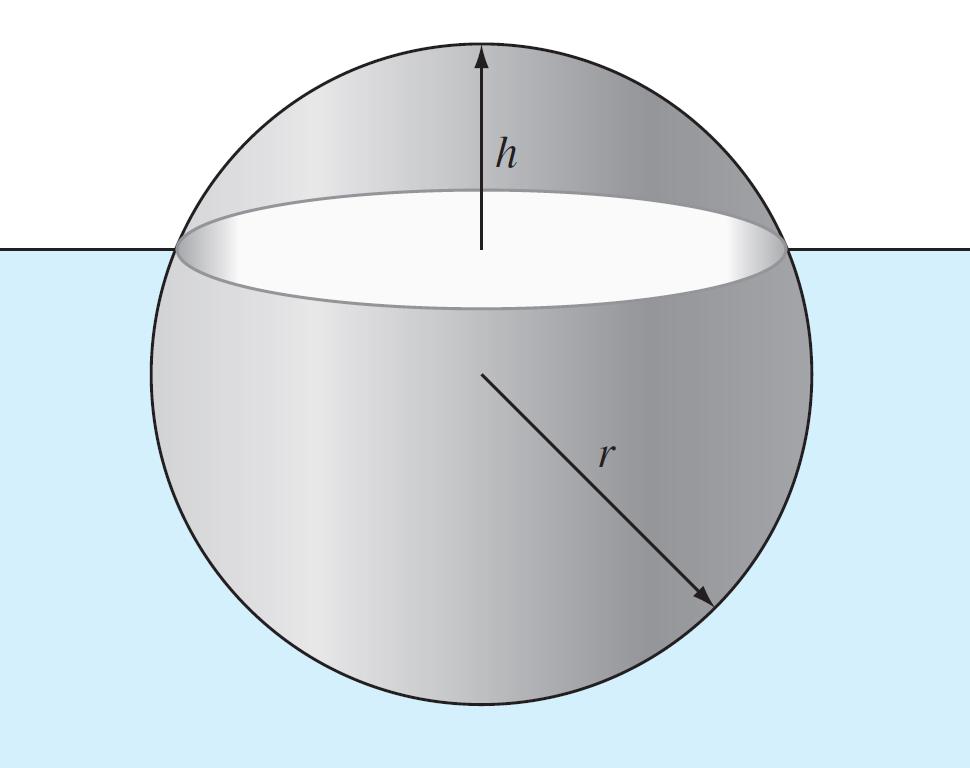
\includegraphics[width=0.8\linewidth]{./images/problem_5_9_4}
        \captionof*{figure}{Figure P5.22}
    \end{minipage}
    \bigskip

    \noindent\textbf{5.23} Perform the same computation as in Prob. 5.22, but for
    the frustrum of a cone as depicted in Fig. P5.23. Employ the
    following values for your computation: $r_1 = 0.5$ m, $r_2= 1$ m,
    $h=1$ m, $\rho_f$ = frustrum density = $200 kg/m^3$, and $\rho_w$ = water
    density = $1,000 kg/m^3$. Note that the volume of a frustrum is given by\\

    $V = \dfrac{\pi h}{3} (r^2_1 + r^2_2 + r_1r_2)$\\

    \noindent
    \begin{minipage}{\linewidth}
        \centering
        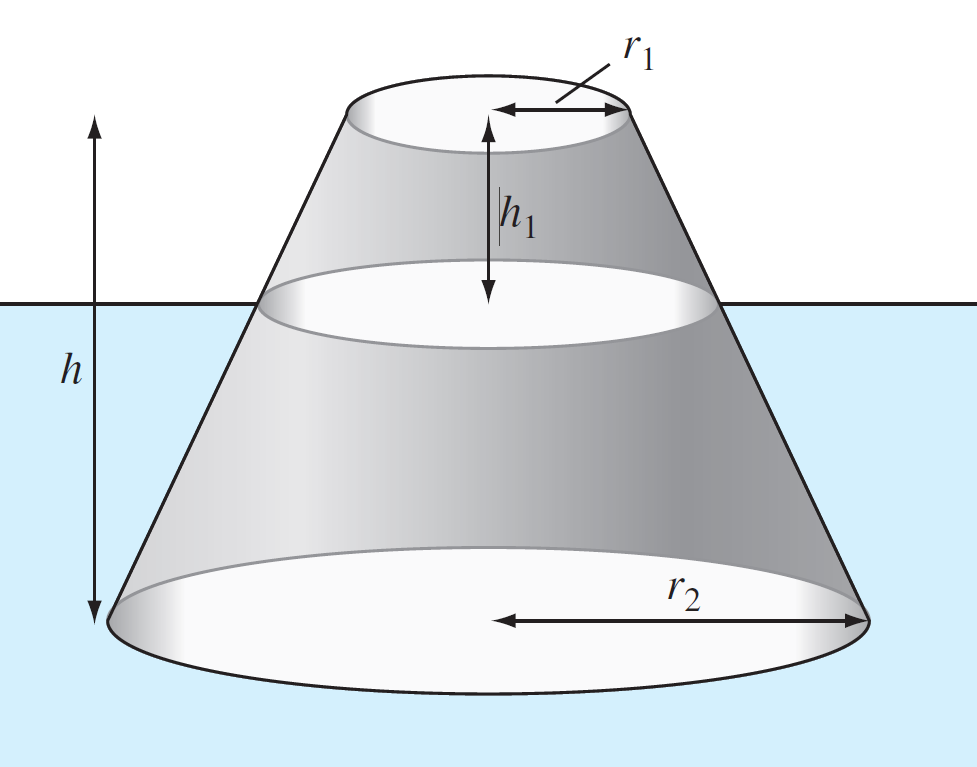
\includegraphics[width=0.8\linewidth]{./images/problem_5_9_5}
        \captionof*{figure}{Figure P5.23}
    \end{minipage}
\end{multicols}

\end{document}